\documentclass[12pt]{article}

\usepackage[a4paper]{geometry}
\usepackage{graphicx} % Required for inserting images
\usepackage{polski} % do znaków polskich
\usepackage[main=polish,english]{babel}
\usepackage{titlesec} % do edycji formatowania sekcji i podsekcji (\titleformat)
\usepackage{blindtext}
\usepackage[T1]{fontenc}
\usepackage{times} % czcionka podstawowa Times New Roman
\usepackage{indentfirst} % wciecia akapitow
\usepackage{amsmath} 
\counterwithin{equation}{section} %numeracja wzorkow 
\usepackage{float} % to jest potrzebne do [H] przy figure
% [H] obok begin{figure} powoduje ze plik jest na pdfie w tym miejscu jak w 
% kodzie, inaczej ustawia sie on jakos na gorze strony albo inaczej
% niz chce
\usepackage{xcolor} % do zmieniania koloru poszczegolnych blokow tekstu
\usepackage{ragged2e} % do wyrownywania tekstu
%\usepackage[none]{hyphenat} % wylaczenie dzielenia wyrazow na koncu wiersza
\usepackage{caption} % pozwala uzywac \\ w opisach grafik
\usepackage{tabularx} % potrzebne do tabelki z danymi
%\usepackage{fixltx2e} % subscripts bez math mode'a, nie jest potrzebne od 2015 xd
\usepackage[hidelinks]{hyperref} % pozwala na interaktywny spis tresci
\usepackage{gensymb} % m.in. dodaje znak stopni
\usepackage{wrapfig} % do umieszczania obrazow w tekscie
\usepackage{subfig}

% ustawienie formatowania sekcji i podsekcji
\titleformat*{\section}{\normalsize\bfseries}
\titleformat*{\subsection}{\normalsize\bfseries}
\titleformat*{\subsubsection}{\normalsize\bfseries}
\titleformat*{\paragraph}{\large\bfseries}
\titleformat*{\subparagraph}{\large\bfseries}
\geometry{lmargin=3.5cm, rmargin=2.5cm, tmargin=2.5cm, bmargin=2.5cm} % marginesy
\setlength\parindent{1cm} % wciecie 
\renewcommand\thesubsubsection{\alph{subsubsection})} % ustawienie a,b,c...
% jako numeracji podpodsekcji

\usepackage{enumitem}
\setlist[enumerate, 1]{label=\textbf{\arabic{*})}} % ustawienie pogrubionej numeracji

\newcommand{\pytanie}[2]{\item \textbf{#1} \\}

\title{Odpowiedzi na pytania do wykładu}
\author{Cezary Karolak}
\date{2023Z}

\begin{document}

\maketitle
\tableofcontents
\newpage

\section{Wykład 1 -- System elektroenergetyczny}
\begin{enumerate}
    \item \textbf{Jakie podstawowe zbiory urządzeń wchodzą w skład systemu elektroenergetycznego?}
    
    \item \textbf{W jaki sposób można dokonać podziału jednostek wytwórczych w elektrowniach?}
    
        Jednostki wytwórcze dzielą się na tradycyjne (węglowe, jądrowe, gazowe, na paliwa płynne) 
        i na wykorzystujące odnawialne źródła energii (wodne, wiatrowe, słoneczne, biogaz i biomasę).

    \item \textbf{Wymienić parametry charakteryzujące system elektroenergetyczny.}
    
        Parametry charakteryzujące SEE:\\
        - moc zainstalowana w jedonstkach wytwórczych,\\
        - moc najwięjszej jednostki wytwórczej,\\
        - moc największej elektrowni,\\
        - najwyższe napięcie znamionowe (nominalne) sieci przesyłowej,\\
        - zapotrzebowanie szczytowne na moc,\\
        - roczna produkcja energii elektrycznej,\\
        - struktura mocy,\\
        - struktura sieci.

    \item \textbf{Podać parametry charakteryzujące strukturę mocy systemu elektroenergetycznego.}
    
        Strukturę mocy charakteryzuje sposób pokrywania obciążeń systemu, zawiera więc dane o jednostkach wytwórczych.

    \item \textbf{Podać jakie elementy wchodzą w skład stacji elektroenergetycznej?}
    
        W stacjach elektroenergetycznych występują następujące elementy:\\
        - transformatory,\\
        - szyny zbiorcze,\\
        - łączniki,\\
        - dławiki,\\
        - baterie kondensatorów,\\
        - inne urządzenia.

    \item \textbf{Wymienić rodzaje sieci i poziomy napięć występujące obecnie w polskich sieciach elektroenergetycznych.}

        Sieci elektroenergetyczne dzieli się na sieci energetyki zawodowej i sieci
        energetyki przemysłowej.\\ Sieci elektroenergetyczne dzieli się na sieci przesyłowe i dystrybucyjne. 
        Sieci przesyłowe to stacje najwyższych napięć (NN), czyli linie o napięciu powyżej 110kV (220kV i 400kV).
        Sieci dystrybucyjne to stacje niskich (nN), średnich (SN) i wysokich (WN) napięć. 
        W Polsce są to:\\
        - nN: 0,4kV i 0,66kV\\
        - SN: 6kV, 10kV, 15kV, 20kV i 30kV\\
        - WN: 110kV
    
    \item \textbf{Wymienić parametry jakościowe energii elektrycznej oraz podać, jaki jest najważniejszy parametr 
    energii elektrycznej, decydujący o pracy systemu elektroenergetycznego?}

        Podstawowe parametry jakościowe energii elektrycznej to:\\
        - częstotliwość,\\
        - napięcie (wartość, poziom),\\
        - symetria fazowa napięć,\\
        - zawartość harmonicznych w krzywej napięcia,\\
        - ciągłość dostawy energii.\\
        Najważniejszy parametr jakościowy to częstotliwość. Zależy ona od zapasu mocy czynnej w jednostkach
        wytwórczych oraz od działania układów automatycznej regulacji częstotliwości w SEE.

    \item \textbf{W którym kraju w Europie jest największy udział OZE w produkcji energii elektrycznej?}

        Największy udział OZE w produkcji energii elektrycznej ma Norwegia - 104,6\%.
        
    \item \textbf{Ile państw w Europie wchodzi w skład (jest członkiem) ENTSO-E?}

        W skład ENTSO-E wchodzi 35 państw członkowskich z 39 operatorów systemów przesyłowych. Państwami mającymi status obserwatora są Turcja i Ukraina.
        
    \item \textbf{Ile wynosiła moc zainstalowana elektrowni w KSE pod koniec 2022 roku?}
    
        Moc zainstalowana elektrowni (łączna moc znamionowa wszystkich jednostek wytwórczych) 
        w KSE (Krajowy System Elektroenergetyczny) pod koniec 2022 roku wynosiła 60446 MW.

    \item \textbf{Wymienić największe polskie elektrownie na węgiel brunatny, na węgiel kamienny, elektrownie wodne oraz elektrownie gazowe.}
    
        Największe polskie elektrownie:\\
        - węgiel brunatny: Bełchatów (5102 MW),\\
        - węgiel kamienny: Kozienice 1+2 (4020 MW),\\
        - wodna pompowa: Żarnowiec (780 MW),\\
        - gazowa: Płock (630 MW).

    \item \textbf{Podać ile wynosiła na koniec 2021 roku sumaryczna długość wszystkich linii napowietrznych 400 kV w Polsce.}
    
        Na koniec 2021 roku sumaryczna długość wszystkich linii napowietrznych 400kV w Polsce wynosiła 8227 km.

\end{enumerate}

\newpage

\section{Wykład 2 -- Jednostki wytwórcze energii elektrycznej}
\begin{enumerate}
    \item \textbf{Omówić cykl przemian energii w elektrowni cieplnej.}

        W wyniku spalania paliwa organiczego lub rozszczepienia paliwa jądrowego otrzymuje się energię cieplną,
        którą przekazujemy do czynnika roboczego (zwykle czynnikiem jest para wodna). Czynnik roboczy wykonuje pracę 
        w silniku cieplnym napędzając tym samym generator prądu. W większości przypadków rolę silnika cieplnego pełni turbina parowa.

    \item \textbf{Podać zasadnicze różnice między układem jednoobiegowym i dwuobiegowym w elektrowni jądrowej.}
    
        W układzie jednobiegowym chłodziwo reaktora (to co odbiera ciepło reaktora) jest również czynnikiem roboczym
        w turbinie (napędza generator).\\
        W układzie dwubiegowym chłodziwo reaktora przekazuje ciepło czynnikowi roboczemu, a elementem sprzęgającym
        oba biegi jest wymiennik ciepła (wytwornica pary).

    \item \textbf{Podać zalety stosowania elektrowni wodnych w stosunku do elektrowni cieplnych.}

        Zalety stosowania elektrowni wodnych w stosunku do elektrowni cieplnych:\\
        - wykorzystują odnawialne zasoby energetyczne przyrody,\\
        - posiadają wysoką sprawność, często przekraczającą 90\%,\\
        - wywierają stosunkowo najmniej destruktywny wpływ na środowisko,\\
        - charakteryzują się szybkim rozruchem i możliwością niemal natychmiastowego pełnego obciążenia.
    
    \item \textbf{Przedstawić podział elektrowni wodnych ze względu na ich konstrukcję.}
    
        Elektrownie wodne ze względu na konstrukcję dzieli się na:\\
        - \underline{przepływowe}: wykorzystują ciągły przepływ wody, nie posiadają zbiornika do jej magazynowania\\
        - \underline{zbiornikowe}: wyposażone w duże zbiorniki umożliwiające gromadzenie dużej ilości wody\\
        - \underline{szczytowo - pompowe}: pełnią rolę magazynów energii. W szczycie obciążenia generują energię elektryczną w wyniku
        przepływu wody ze zbiornika górnego do dolnego. W okresie zmniejszonego zapotrzebowania na moc przepompowują
        wodę ze zbiornika dolnego do górnego.

    \item \textbf{Sklasyfikować jednostki generacji rozproszonej pod względem mocy zainstalowanej.}

        Podział jednostek generacji rozproszonej pod względem mocy zainstalowanej:\\
        - mikrogeneracja rozproszona - od 1 W do 5 kW\\
        - mała generacja rozproszona - od 1 kW do 5 MW\\
        - średnia generacja rozproszona - od 5 MW do 50 MW\\
        - duża generacja rozproszona - od 50 MW do 150 MW
        
    \pytanie{Podać główne zalety i wady elektrowni wiatrowych.}

        Zalety elektrowni wiatrowych:\\
        - wykorzystanie niewyczerpalnych zasobów energii\\
        - brak emisji szkodliwych substancji do środowiska\\
        Wady elektrowin wiatrowych:\\
        - emisja hałasu podczas pracy\\
        - wywołanie zakłóceń elektromagnetycznych\\
        - duża zajętość terenu\\
        - szpecenie krajobrazu\\
        - zagrożenie dla ptaków\\
        - praca uzależniona od prędkości wiatru
        
    \item \textbf{Wyjaśnić różnicę pomiędzy systemami fotowoltaicznymi off-grid i ongrid.}
    \item \textbf{Wyjaśnić zasadę działania i cechy charakterystyczne spalinowego silnika tłokowego.}
    \item \textbf{Narysować i omówić schemat ideowy przyłączenia mikroturbiny do sieci elektroenergetycznej.}
\end{enumerate}

\section{Wykład 7 -- Moc i energia w systemie elektroenergetycznym}
\begin{enumerate}
    \pytanie{Przedstaw trójkąt mocy i wynikające z niego zależności pomiędzy występującymi 
    w nim mocami.}

        \begin{figure}[H]
            \centering
            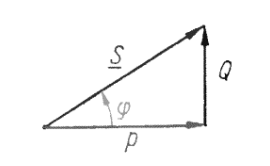
\includegraphics[width=0.3\linewidth]{images/wyklad7_1.png}
            \caption*{Trójkąt mocy}
        \end{figure}
        \begin{equation*}
            P = S \cdot \cos\varphi
        \end{equation*}
        \begin{equation*}
            Q = S \cdot \sin\varphi
        \end{equation*}
        \begin{equation*}
            S = P + jQ
        \end{equation*}

    \pytanie{Wyjaśnij, z czym silnie związane są zmiany mocy czynnej i biernej w systemie 
    elektroenergetycznym.}

        Wpływając na wartość mocy czynnej jednocześnie wpływa się mocno na kąt mocy ($\delta$) i odwrotnie.
        Wpływając na wartość mocy biernej jednocześnie wpływa się na wartość napięcia.
        Wynika to z poniższych wzorów:
        \begin{equation*}
            P = U I \cos\varphi = \frac{E U}{X} \sin\delta
        \end{equation*}
        \begin{equation*}
            Q = U I \sin\varphi = \frac{E U}{X} \cos\delta - \frac{U^2}{X}
        \end{equation*}

    \pytanie{Przedstaw główne odbiorniki mocy biernej.}

        

    \pytanie{Przedstaw model obwodowy linii elektroenergetycznej wysokiego napięcia.}

    \pytanie{Do czego służy energetyczny równoważnik mocy biernej?}

    \pytanie{Przedstaw negatywne skutki przesyłania mocy biernej przez sieć 
    elektroenergetyczną.}

    \pytanie{Wyjaśnij, za pomocą odpowiedniego wzoru, dlaczego obecność mocy biernej 
    zmniejsza zdolność przepustową linii elektroenergetycznych.}

    \pytanie{Przedstaw naturalne i sztuczne metody kompensacji mocy biernej.}

    \pytanie{Podaj zalety i wady stosowania kondensatorów do kompensacji mocy biernej.}

    \pytanie{Przedstaw możliwe rodzaje kompensacji mocy biernej w zależności od miejsca 
    instalacji baterii kondensatorów.}

    \pytanie{Który rodzaj kompensacji mocy biernej jest najbardziej skuteczny, a który 
    najmniej? Odpowiedź uzasadnij.}

    \pytanie{Jaki jest wzór na moc baterii do centralnej kompensacji mocy biernej?}

    \pytanie{Przedstaw metody zmniejszania strat mocy w sieci elektroenergetycznej.}

\end{enumerate}



\end{document}
